\documentclass[
  shownotes,
  xcolor={svgnames},
  hyperref={colorlinks,citecolor=DarkBlue,linkcolor=DarkRed,urlcolor=DarkBlue}
  , aspectratio=169]{beamer}
\usepackage{animate}
\usepackage{amsmath}
\usepackage{amsfonts}
\usepackage{amssymb}
\usepackage{pifont}
\usepackage{mathpazo}
%\usepackage{xcolor}
\usepackage{multimedia}
\usepackage{fancybox}
\usepackage[para]{threeparttable}
\usepackage{multirow}
\setcounter{MaxMatrixCols}{30}
\usepackage{subcaption}
\usepackage{graphicx}
\usepackage{lscape}
\usepackage[compatibility=false,font=small]{caption}
\usepackage{booktabs}
\usepackage{ragged2e}
\usepackage{chronosys}
\usepackage{appendixnumberbeamer}
\usepackage{animate}
\setbeamertemplate{caption}[numbered]
\usepackage{color}
%\usepackage{times}
\usepackage{tikz}
\usepackage{comment} %to comment
%% BibTeX settings
\usepackage{natbib}
\bibliographystyle{apalike}
\bibpunct{(}{)}{,}{a}{,}{,}
\setbeamertemplate{bibliography item}{[\theenumiv]}

% Defines columns for bespoke tables
\usepackage{array}
\newcolumntype{L}[1]{>{\raggedright\let\newline\\\arraybackslash\hspace{0pt}}m{#1}}
\newcolumntype{C}[1]{>{\centering\let\newline\\\arraybackslash\hspace{0pt}}m{#1}}
\newcolumntype{R}[1]{>{\raggedleft\let\newline\\\arraybackslash\hspace{0pt}}m{#1}}


\usepackage{xfrac}


\usepackage{multicol}
\setlength{\columnsep}{0.5cm}

% Theme and colors
\usetheme{Boadilla}

% I use steel blue and a custom color palette. This defines it.
\definecolor{andesred}{HTML}{af2433}

% Other options
\providecommand{\U}[1]{\protect\rule{.1in}{.1in}}
\usefonttheme{serif}
\setbeamertemplate{itemize items}[default]
\setbeamertemplate{enumerate items}[square]
\setbeamertemplate{section in toc}[circle]

\makeatletter

\definecolor{mybackground}{HTML}{82CAFA}
\definecolor{myforeground}{HTML}{0000A0}

\setbeamercolor{normal text}{fg=black,bg=white}
\setbeamercolor{alerted text}{fg=red}
\setbeamercolor{example text}{fg=black}

\setbeamercolor{background canvas}{fg=myforeground, bg=white}
\setbeamercolor{background}{fg=myforeground, bg=mybackground}

\setbeamercolor{palette primary}{fg=black, bg=gray!30!white}
\setbeamercolor{palette secondary}{fg=black, bg=gray!20!white}
\setbeamercolor{palette tertiary}{fg=white, bg=andesred}

\setbeamercolor{frametitle}{fg=andesred}
\setbeamercolor{title}{fg=andesred}
\setbeamercolor{block title}{fg=andesred}
\setbeamercolor{itemize item}{fg=andesred}
\setbeamercolor{itemize subitem}{fg=andesred}
\setbeamercolor{itemize subsubitem}{fg=andesred}
\setbeamercolor{enumerate item}{fg=andesred}
\setbeamercolor{item projected}{bg=gray!30!white,fg=andesred}
\setbeamercolor{enumerate subitem}{fg=andesred}
\setbeamercolor{section number projected}{bg=gray!30!white,fg=andesred}
\setbeamercolor{section in toc}{fg=andesred}
\setbeamercolor{caption name}{fg=andesred}
\setbeamercolor{button}{bg=gray!30!white,fg=andesred}


\usepackage{fancyvrb}
\newcommand{\VerbBar}{|}
\newcommand{\VERB}{\Verb[commandchars=\\\{\}]}
\DefineVerbatimEnvironment{Highlighting}{Verbatim}{commandchars=\\\{\}}
% Add ',fontsize=\small' for more characters per line
\usepackage{framed}
\definecolor{shadecolor}{RGB}{248,248,248}
\newenvironment{Shaded}{\begin{snugshade}}{\end{snugshade}}
\newcommand{\AlertTok}[1]{\textcolor[rgb]{0.94,0.16,0.16}{#1}}
\newcommand{\AnnotationTok}[1]{\textcolor[rgb]{0.56,0.35,0.01}{\textbf{\textit{#1}}}}
\newcommand{\AttributeTok}[1]{\textcolor[rgb]{0.77,0.63,0.00}{#1}}
\newcommand{\BaseNTok}[1]{\textcolor[rgb]{0.00,0.00,0.81}{#1}}
\newcommand{\BuiltInTok}[1]{#1}
\newcommand{\CharTok}[1]{\textcolor[rgb]{0.31,0.60,0.02}{#1}}
\newcommand{\CommentTok}[1]{\textcolor[rgb]{0.56,0.35,0.01}{\textit{#1}}}
\newcommand{\CommentVarTok}[1]{\textcolor[rgb]{0.56,0.35,0.01}{\textbf{\textit{#1}}}}
\newcommand{\ConstantTok}[1]{\textcolor[rgb]{0.00,0.00,0.00}{#1}}
\newcommand{\ControlFlowTok}[1]{\textcolor[rgb]{0.13,0.29,0.53}{\textbf{#1}}}
\newcommand{\DataTypeTok}[1]{\textcolor[rgb]{0.13,0.29,0.53}{#1}}
\newcommand{\DecValTok}[1]{\textcolor[rgb]{0.00,0.00,0.81}{#1}}
\newcommand{\DocumentationTok}[1]{\textcolor[rgb]{0.56,0.35,0.01}{\textbf{\textit{#1}}}}
\newcommand{\ErrorTok}[1]{\textcolor[rgb]{0.64,0.00,0.00}{\textbf{#1}}}
\newcommand{\ExtensionTok}[1]{#1}
\newcommand{\FloatTok}[1]{\textcolor[rgb]{0.00,0.00,0.81}{#1}}
\newcommand{\FunctionTok}[1]{\textcolor[rgb]{0.00,0.00,0.00}{#1}}
\newcommand{\ImportTok}[1]{#1}
\newcommand{\InformationTok}[1]{\textcolor[rgb]{0.56,0.35,0.01}{\textbf{\textit{#1}}}}
\newcommand{\KeywordTok}[1]{\textcolor[rgb]{0.13,0.29,0.53}{\textbf{#1}}}
\newcommand{\NormalTok}[1]{#1}
\newcommand{\OperatorTok}[1]{\textcolor[rgb]{0.81,0.36,0.00}{\textbf{#1}}}
\newcommand{\OtherTok}[1]{\textcolor[rgb]{0.56,0.35,0.01}{#1}}
\newcommand{\PreprocessorTok}[1]{\textcolor[rgb]{0.56,0.35,0.01}{\textit{#1}}}
\newcommand{\RegionMarkerTok}[1]{#1}
\newcommand{\SpecialCharTok}[1]{\textcolor[rgb]{0.00,0.00,0.00}{#1}}
\newcommand{\SpecialStringTok}[1]{\textcolor[rgb]{0.31,0.60,0.02}{#1}}
\newcommand{\StringTok}[1]{\textcolor[rgb]{0.31,0.60,0.02}{#1}}
\newcommand{\VariableTok}[1]{\textcolor[rgb]{0.00,0.00,0.00}{#1}}
\newcommand{\VerbatimStringTok}[1]{\textcolor[rgb]{0.31,0.60,0.02}{#1}}
\newcommand{\WarningTok}[1]{\textcolor[rgb]{0.56,0.35,0.01}{\textbf{\textit{#1}}}}
\usepackage{graphicx}
\makeatletter

\definecolor{airforceblue}{rgb}{0.36, 0.54, 0.66}

\usepackage{tikz}
% Tikz settings optimized for causal graphs.
\usetikzlibrary{shapes,decorations,arrows,calc,arrows.meta,fit,positioning}
\tikzset{
    -Latex,auto,node distance =1 cm and 1 cm,semithick,
    state/.style ={ellipse, draw, minimum width = 0.7 cm},
    point/.style = {circle, draw, inner sep=0.04cm,fill,node contents={}},
    bidirected/.style={Latex-Latex,dashed},
    el/.style = {inner sep=2pt, align=left, sloped}
}


\makeatother






%%%%%%%%%%%%%%% BEGINS DOCUMENT %%%%%%%%%%%%%%%%%%

\begin{document}

\title[Lecture 17]{Lecture 17: \\ Regularization/Shrinkage Methods}
\subtitle{Big Data and Machine Learning for Applied Economics \\ Econ 4676}
\date{\today}

\author[Sarmiento-Barbieri]{Ignacio Sarmiento-Barbieri}
\institute[Uniandes]{Universidad de los Andes}


\begin{frame}[noframenumbering]
\maketitle
\end{frame}

%%%%%%%%%%%%%%%%%%%%%%%%%%%%%%%%%%%



%----------------------------------------------------------------------% 

\begin{frame}
\frametitle{Agenda}

\tableofcontents

\end{frame}

%----------------------------------------------------------------------%
\section{Recap: Model Selection}
%----------------------------------------------------------------------%
\begin{frame}[fragile]
\frametitle{Model Selection}


\begin{itemize}
  \item ML we care about prediction out of sample
  \medskip
  \begin{align}
  y= \beta_0 + \beta_1 X_1 + \beta_2 X_2 + \dots + \beta_{k-1} X_{k-1} + \beta_k X_k + u 
  \end{align}
  \medskip
  \item Trade off Bias/Variance: more "complex" models have less bias but more variance
  \medskip
  \item Overfit: complex models predict very well inside a sample but "bad" outside
  \medskip
  \item Choose the right complexity level
  \medskip
  \item Big innovation accept some bias to decrease variance $\rightarrow$ improves out of sample prediction
\end{itemize}

\end{frame}

%----------------------------------------------------------------------%
\begin{frame}[fragile]
\frametitle{Model Selection}

\begin{itemize}
\item Given the models, we choose the one that ``best'' predicts out of sample
\medskip
\begin{align}
  M_0 &\rightarrow y= \beta_0  + u  \\ 
  M_1 &\rightarrow y= \beta_0  + \beta_j X_j +u \\
  \vdots \\
  M_k &\rightarrow y= \beta_0   + \beta_1 X_1 + \beta_2 X_2 + \dots + \beta_k X_k +u 
  \end{align}
  \medskip

  \item How we bet the ``best'': 
  \medskip
\begin{enumerate}
  \item Choose based on some measure of sample fit, but penalized for complexity, e.g. $BIC=SSR - \frac{1}{2}p \log(n)$
  \medskip
  \item Use resampling techniques (create ``a fake'' out of sample) use prediction error
\end{enumerate}


\end{itemize}

\end{frame}
%----------------------------------------------------------------------%
\begin{frame}[fragile]
\frametitle{Model Selection}

\begin{itemize}
\item Where do these $k$ models come from? If I have $k$ variables how do I search among the possible models
\medskip
\begin{align}
  M_0 &\rightarrow y= \beta_0  + u  \\ 
  M_1 &\rightarrow y= \beta_0  + \beta_j X_j +u \\
  \vdots \\
  M_k &\rightarrow y= \beta_0   + \beta_1 X_1 + \beta_2 X_2 + \dots + \beta_k X_k +u 
  \end{align}
\medskip 

\item  Best subset selection
\medskip 
\item Forward  Stepwise Selection
\medskip 
\item Backward Stepwise Selection
\end{itemize}
\end{frame}
%----------------------------------------------------------------------%
\section{Regularization}
%----------------------------------------------------------------------%
\begin{frame}[fragile]
\frametitle{Regularization}


\begin{itemize}
  \item What about if I do the following?
\medskip
\item Get the most general model I can
  \begin{align}
  y= \beta_0 + \beta_1 X_1 + \beta_2 X_2 + \dots + \beta_{k-1} X_{k-1} + \beta_k X_k + u 
  \end{align}
\pause
\medskip
\begin{itemize}
    \item Run model, get coefficients and p-values
    \medskip
    \pause
    \item Take out those with p-values bellow a certain $\alpha$
    \medskip
    \pause
    \item Why is this a bad idea?
\end{itemize}
\medskip
\pause
\item Backward selection approximates that idea (not exactly) and does a better job that the previous point.
\end{itemize}
\end{frame}
%----------------------------------------------------------------------%
\begin{frame}[fragile]
\frametitle{Regularization}

\begin{itemize}
  \item 'Crossing out' variables / coefficients is an extreme way to 'shrink' them. 
  \medskip
  \item Lasso: a formal and algorithmic way of accomplishing this task. 
  \medskip
  \item The strategy involves penalizing complexity so as to depart from optimality and stabilize the system
  \medskip
  \item The key of modern statistics is regularization


\end{itemize}
 

\end{frame}
%----------------------------------------------------------------------%
\subsection{Lasso}
%----------------------------------------------------------------------%
\begin{frame}[fragile]
\frametitle{Lasso}

\begin{itemize}
\item For $\lambda \geq 0$ given, consider minimizing the following objective function


\begin{align}
min_{\beta} L(\beta) = \sum_{i=1}^n (y_i-x_i'\beta)^2 + \lambda \sum_{s=2}^p |\beta_s| 
\end{align}

\bigskip
\item Note:
\begin{itemize}
  \item First coef. constant
  \pause
  \item $\lambda = 0$?
  \pause
  \item $\lambda = \infty$?
\end{itemize}
\end{itemize}
\end{frame}

%----------------------------------------------------------------------%
\begin{frame}[fragile]
\frametitle{Lasso}

\begin{align}
min_{\beta} L(\beta) = \sum_{i=1}^n (y_i-x_i'\beta)^2 + \lambda \sum_{s=2}^p |\beta_s| 
\end{align}
\bigskip
\begin{itemize}
\item  LASSO's free lunch: automatically chooses which variables go in ($\beta_s \neq 0$) and which are out  ($\beta_s = 0$)
\medskip
\item Why? Coefficients that don't go in  are corner solutions 
\medskip
\item  $L(\beta)$ in non differentiable
\end{itemize}

\end{frame}
%----------------------------------------------------------------------%
\begin{frame}[fragile]
\frametitle{Corner Solutions}

\begin{itemize}
\item Lasso Intuition
\end{itemize}

\bigskip

\begin{align}
min_{\beta} L(\beta) = \sum_{i=1}^n (y_i-x_i \beta)^2 + \lambda|\beta| 
\end{align}

\begin{itemize}
  \item Only one predictor, i.e., one coefficient.
  \medskip
  \item For $\lambda=0$

  \begin{align}
    \hat{\beta}_{OLS}= \frac{\sum_i x_i y_i}{\sum_i x_i^2}
  \end{align}
  \item If we standardize predictor $\sum x_i^2=1$?
\end{itemize}




\end{frame}
%----------------------------------------------------------------------%
\begin{frame}[fragile]
\frametitle{Corner Solutions}

\begin{align}
min_{\beta} L(\beta) = \sum_{i=1}^n (y_i-x_i \beta)^2 + \lambda|\beta| 
\end{align}
\begin{itemize}
  \item Non differentiable at $\beta=0$
  \item Differentiable otherwise $\beta\neq0$
\end{itemize}

\begin{align}
L(\beta)=\sum_{i=1}^{n}(y_{i}-x_{i}\beta)^{2}+\lambda|\beta|=\begin{cases}
\sum_{i=1}^{n}(y_{i}-x_{i}\beta)^{2}+\lambda\beta & if\,\,\beta>0\\
\sum_{i=1}^{n}(y_{i}-x_{i}\beta)^{2}-\lambda\beta & if\,\,\beta<0
\end{cases}
\end{align}


\end{frame}
%----------------------------------------------------------------------%
\begin{frame}[fragile]
\frametitle{Corner Solutions}

   \begin{figure}[H] \centering
            \captionsetup{justification=centering}
              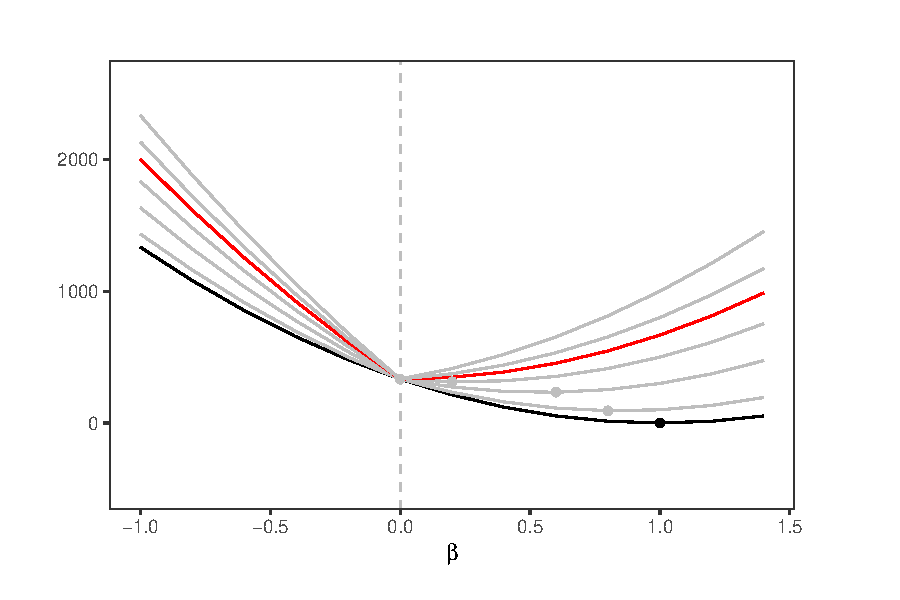
\includegraphics[scale=0.8]{figures/lasso.pdf}
 \end{figure}

 \end{frame}
%----------------------------------------------------------------------%
\begin{frame}[fragile]
\frametitle{Corner Solutions}

\begin{align}
\frac{dL(\beta)^+}{d\beta} &= -2 \sum y_ix_i+ 2 \beta \sum x_i^2 + \lambda \nonumber \\
& = -2 \sum y_ix_i +\beta + \lambda
\end{align}

\begin{align}
\frac{dL(0)^+}{d\beta} &= -2 \sum y_ix_i + \lambda \nonumber 
\end{align}

then, if 

\begin{align}
   \lambda \geq 2 \sum y_ix_i 
\end{align}

we have $\hat{\beta}_{lasso}=0$

 \end{frame}
%----------------------------------------------------------------------%
\begin{frame}[fragile]
\frametitle{Corner Solutions}

\begin{itemize}


\item If  $\lambda < 2 \sum y_ix_i $ we have an interior solution

\begin{align}
  -2 \sum y_ix_i + \hat{\beta}_{lasso} + \lambda =0
\end{align}

\medskip
\begin{align}
    \hat{\beta}_{lasso} =\sum y_ix_i  - \frac{\lambda}{2}
\end{align}

\medskip
\begin{align}
    \hat{\beta}_{lasso} =  \hat{\beta}_{OLS} - \frac{\lambda}{2}
\end{align}

\item We get \textcolor{andesred}{shrinkage towards 0}
\end{itemize}


 \end{frame}
%----------------------------------------------------------------------%
\begin{frame}[fragile]
\frametitle{Corner Solutions}

\begin{align}
min_{\beta} L(\beta) = \sum_{i=1}^n (y_i-x_i \beta)^2 + \lambda|\beta| 
\end{align}

\medskip
\begin{align}
\hat{\beta}_{lasso}=\begin{cases}
0 & \text{\text{si} }\ensuremath{\lambda\geq2\sum y_{i}x_{i}}\\
\hat{\beta}_{OLS}-\frac{\lambda}{2} & \text{\text{si} }\ensuremath{\lambda<2\sum y_{i}x_{i}}
\end{cases}
\end{align}



 \end{frame}
%----------------------------------------------------------------------%
\subsection{Ridge}
%----------------------------------------------------------------------%
\begin{frame}[fragile]
\frametitle{Ridge}

\begin{itemize}
\item For $\lambda \geq 0$ given, consider minimizing the following objective function


\begin{align}
min_{\beta} R(\beta) = \sum_{i=1}^n (y_i-x_i'\beta)^2 + \lambda \sum_{s=2}^p (\beta_s)^2
\end{align}

\bigskip
\item Note:
\begin{itemize}
  \item Intuition is similar to Lasso, however the problem is completely different
\end{itemize}
\end{itemize}


\end{frame}
%----------------------------------------------------------------------%
\begin{frame}[fragile]
\frametitle{Ridge}

Simple case 1 predictor

\begin{align}
min_{\beta} R(\beta) = \sum_{i=1}^n (y_i-x_i'\beta)^2 + \lambda  (\beta_s)^2
\end{align}

FOC

\begin{align}
-2 \sum_{i=1}^n  y_i x_i + 2\beta + 2 \lambda  \beta_s =0
\end{align}

\begin{align}
\hat{\beta}_{ridge} &= \frac{\sum_{i=1}^n  y_i x_i}{(1+ \lambda)} \nonumber \\
                    &= \frac{\beta_{OLS}}{(1+ \lambda)}
\end{align}

\begin{itemize}
\item Solution is {\it always} interior (unlike Lasso)
\item Solutions is "shrunken"
\end{itemize}
\end{frame}

%----------------------------------------------------------------------%
\begin{frame}[fragile]
\frametitle{Lasso and Ridge Intuition}

   \begin{figure}[H] \centering
            \captionsetup{justification=centering}
              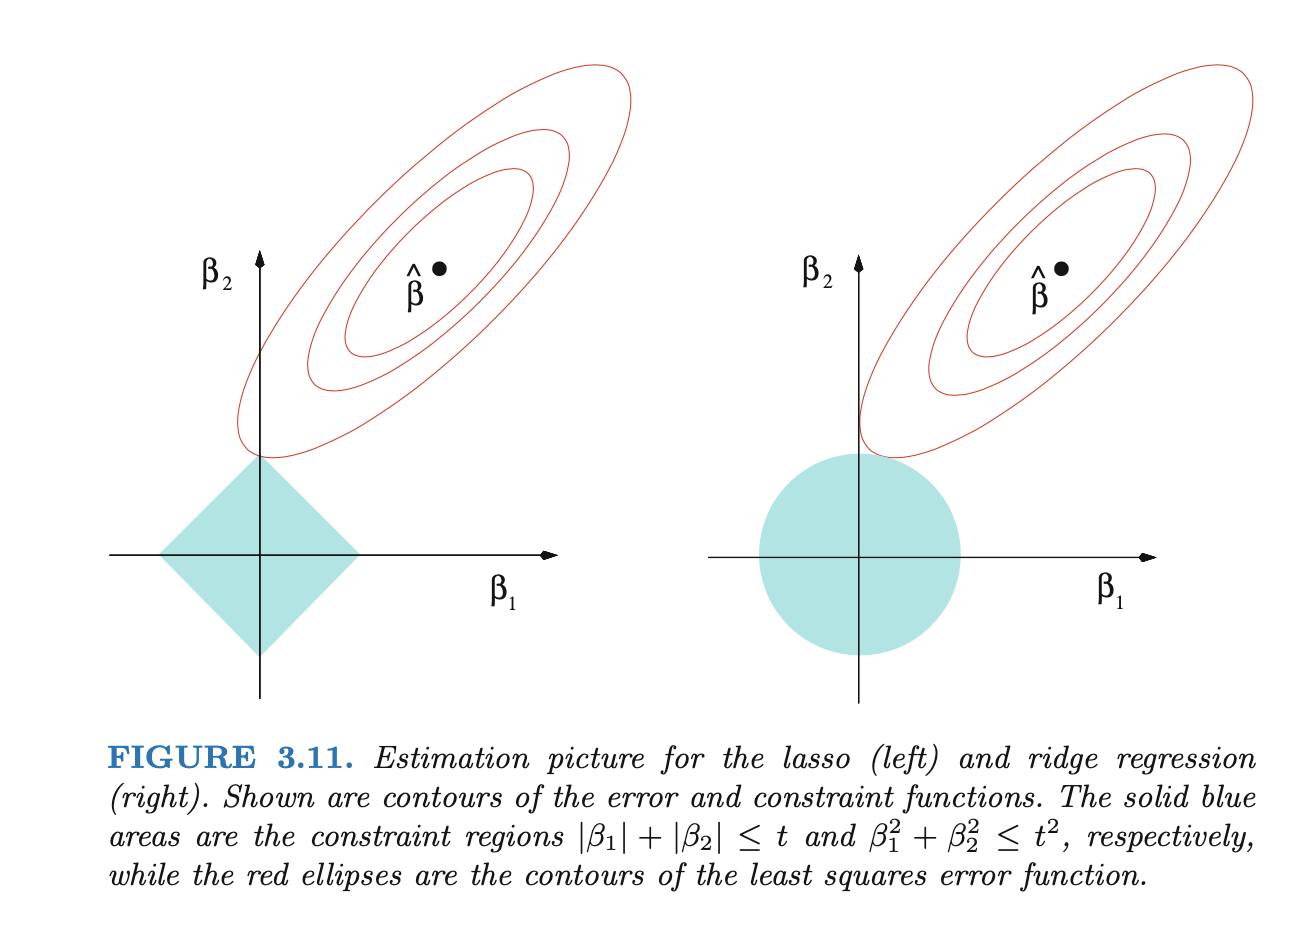
\includegraphics[scale=0.4]{figures/lasso_ridge}
 \end{figure}



\end{frame}
%----------------------------------------------------------------------%
\begin{frame}[fragile]
\frametitle{Lasso and Ridge Example}

   \begin{figure}[H] \centering
            \captionsetup{justification=centering}
              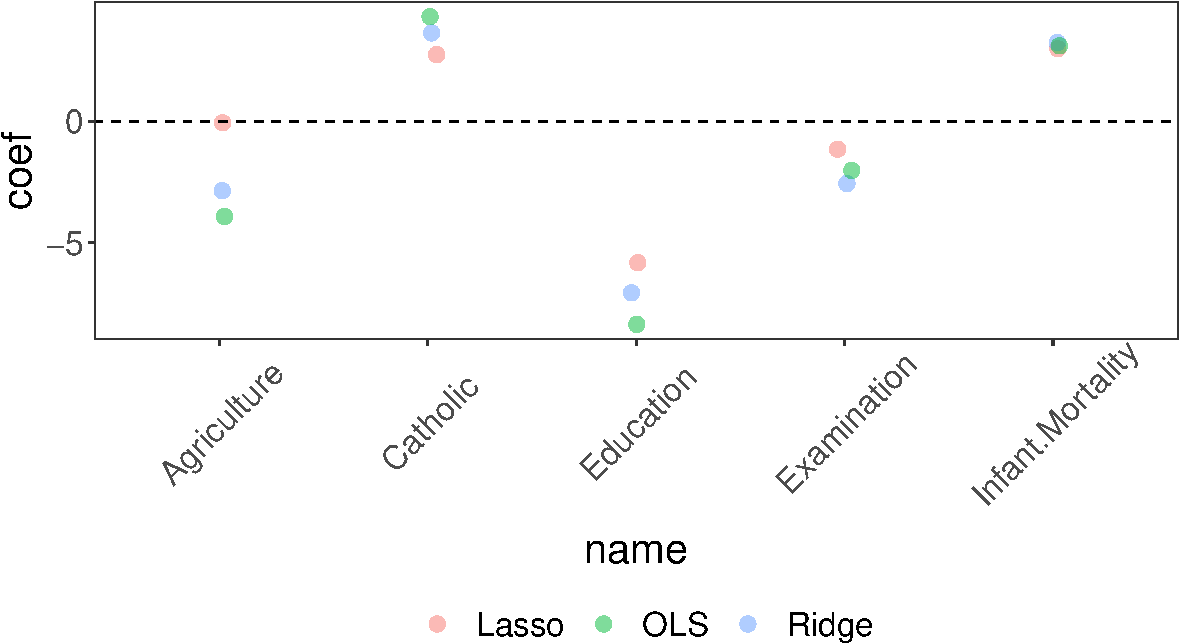
\includegraphics[scale=0.6]{figures/comp}
 \end{figure}

 \end{frame}
%----------------------------------------------------------------------%
\begin{frame}[fragile]
\frametitle{Technical comments}

\begin{itemize}
 \item We showed that Ridge is biased, but you have to show in the PS that $\lambda$ $MSE(\beta_{ridge})<MSE(\beta_{OLS})$
 \medskip
 \item Not possible to derive an exact result for Lasso, but Ridge works similarly
 \medskip
 \item Lasso shrinks everything towards zero, Ridge not quite so
 \medskip
 \item Application wise:
\begin{itemize}
  \medskip
 \item Standardize the data
 \medskip
 \item Selection of $\lambda$?
\end{itemize}
\end{itemize}

 \end{frame}
%----------------------------------------------------------------------%
\begin{frame}[fragile]
\frametitle{Technical comments: $\lambda$ Selection}
\begin{itemize}
 \item Selection of $\lambda$?
 \bigskip
 \item Use CV
 \bigskip
 \begin{itemize}
 \item Choose a grid of $\lambda$ values, and compute the CV error for each value
 \medskip
 \item Select the $\lambda^*$ that minimizes the prediction error
 \medskip
 \item Estimate using all the observations and the selected $\lambda^*$
\end{itemize}
\end{itemize}



\end{frame}

%----------------------------------------------------------------------%
\section{Family of penalized regressions}
%----------------------------------------------------------------------%
\begin{frame}[fragile]
\frametitle{Family of penalized regressions}

\begin{itemize}
\item Family of penalized regressions

\begin{align}
min_{\beta} R(\beta) = \sum_{i=1}^n (y_i-x_i'\beta)^2 + \lambda \sum_{s=2}^p |\beta_s|^p
\end{align}

 \begin{figure}[H] \centering
            \captionsetup{justification=centering}
              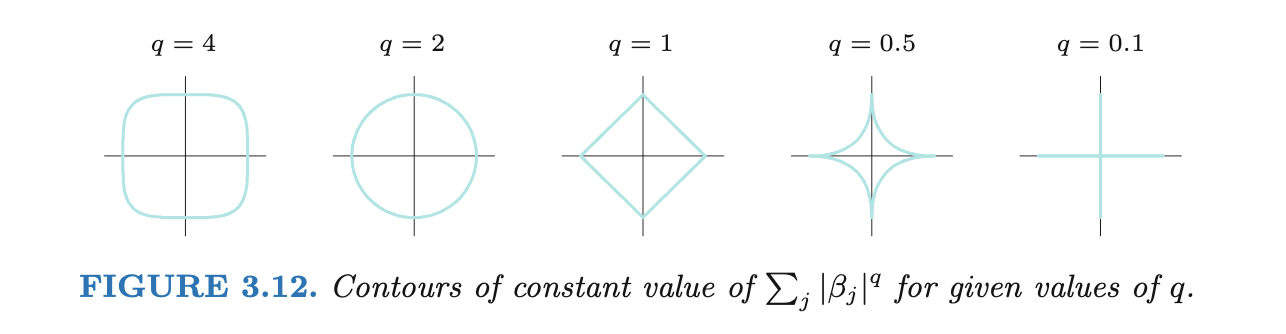
\includegraphics[scale=0.4]{figures/penalties.png}
 \end{figure}
\end{itemize}
\end{frame}
%----------------------------------------------------------------------%
\section{More predictors than observations ($k>n$)}
%----------------------------------------------------------------------%
\begin{frame}[fragile]
\frametitle{More predictors than observations ($k>n$)}

\begin{itemize}
  \item Objective 1: Accuracy
  \begin{itemize}
    \item Minimize prediction error (in one step) $\rightarrow$ Ridge, Lasso
    \end{itemize}
    \medskip
  \item Objective 2: Dimensionality
  \begin{itemize}
    \item Reduce the predictor space $\rightarrow$ Lasso's free lunch
    \end{itemize}
\end{itemize}
\medskip
\pause
\begin{itemize}
  \item What happens when we have more predictors than observations ($k>n$)?
  \begin{itemize}
   \item OLS fails
   \medskip
   \item Ridge and Lasso to the rescue?
  \end{itemize}
\end{itemize}

\end{frame}


%----------------------------------------------------------------------%
\begin{frame}[fragile]
\frametitle{OLS when $k>n$}

\begin{itemize}
  \item Rank? Max number of rows or columns that are linearly independent
  \begin{itemize}
  \item Implies $rank(X_{k\times n}) \leq min(k,n)$
  \end{itemize}
  \bigskip
  \item MCO we need $rank(X_{k\times n})=k \implies k\leq n$
  \bigskip
  \item If $rank(X_{k\times n})=k$ then $rank(X'X)=k$
  \bigskip
  \item If $k>n$, then  $rank(X'X)\leq n < k$ then $(X'X)$ cannot be inverted
  \bigskip
  \item Ridge and Lasso work when $k \geq n$
\end{itemize}

\end{frame}


%----------------------------------------------------------------------%
\begin{frame}[fragile]
\frametitle{Ridge when $k>n$}

\begin{align}
min_{\beta} R(\beta) = \sum_{i=1}^n (y_i-x_i'\beta)^2 + \lambda \sum_{s=1}^p (\beta_s)^2
\end{align}

\bigskip
\begin{itemize}
  \item Solution $\rightarrow$ data augmentation
  \medskip
  \item Intuition: Ridge ``adds'' $k$ additional points.
  \medskip
  \item Allows us to ``deal'' with $k\geq n$
\end{itemize}

\end{frame}
%----------------------------------------------------------------------%
\begin{frame}[fragile]
\frametitle{Lasso when $k>n$}

\begin{itemize}
  \item Lasso works fine in this case
  \medskip
  \item However, there are some issues to keep in mind
  \begin{itemize}
    \medskip
  \item When $k>n$ chooses at most $n$ variables
  \medskip
  \item When we have a group of highly correlated variables, 
  \medskip
    \begin{itemize}
      \item Lasso chooses only one. Makes it unstable for prediction. (Doesn't happen to Ridge)
      \medskip
      \item Ridge shrinks the coefficients of correlated variables toward each other. This makes Ridge ``work'' better than Lasso. ``Work'' in terms of prediction error
    \end{itemize}
  \end{itemize}  
  \medskip
  
\end{itemize}



\end{frame}

%----------------------------------------------------------------------%
\section{Elastic Net}
%----------------------------------------------------------------------%
 \begin{frame}[fragile]
\frametitle{Naive Elastic Net}

\begin{itemize}
\item  Combination? Elastic Net

\begin{align}
min_{\beta} EL(\beta) &= \sum_{i=1}^n (y_i-x_i'\beta)^2 + \lambda_1 \sum_{s=2}^p |\beta_s| + \lambda_2 \sum_{s=2}^p \beta_s^2 \nonumber \\
 &= \sum_{i=1}^n (y_i-x_i'\beta)^2 + \lambda \sum_{s=2}^p \left(  (1-\alpha) \beta_s^2 + \alpha  |\beta_s|\right)
\end{align}

\end{itemize}
\end{frame}


%----------------------------------------------------------------------%
\begin{frame}[fragile]
\frametitle{Naive Elastic Net}

\begin{itemize}
\item Elastic net: happy medium. 
  \begin{itemize}
    \item Good job at prediction and selecting variables
  \end{itemize}
\end{itemize}

\begin{align}
min_{\beta} NEL(\beta) &= \sum_{i=1}^n (y_i-x_i'\beta)^2 + \lambda_1 \sum_{s=2}^p |\beta_s| + \lambda_2 \sum_{s=2}^p \beta_s^2 
\end{align}


\begin{itemize}
 \item Mixes Ridge and Lasso
 \item Lasso selects predictors
 \item Strict convexity part  of the penalty (ridge) solves the grouping instability problem 
 \scriptsize
 \item H.W.: $\beta_{OLS}>0$ one predictor standarized
 \begin{align}
\hat{\beta}_{naive\,EN}= \frac{\left(\hat{\beta}_{OLS}-\frac{\lambda_1}{2}\right)_{+}}{1+\lambda_2}
\end{align}
\end{itemize}

%The second term encourages highly correlated features to be averaged, while the first term encourages a sparse solution in the coefficients of these averaged features. The elastic net penalty can be used with any linear model, in particular for regression or classification. pg 662 Elements
\end{frame}

%----------------------------------------------------------------------%
\begin{frame}[fragile]
\frametitle{Elastic Net}

\begin{itemize}
\item Elastic Net: reescaled version
\item Double Shrinkage introduces ``too'' much bias, {\it final} version ``corrects'' for this
\end{itemize}
\bigskip
\begin{align}
\hat{\beta}_{EN}= \frac{1}{\sqrt{1+\lambda_2}}\hat{\beta}_{naive\,EN}
\end{align}
\bigskip
\begin{itemize}
  \item Careful sometimes software asks.
  \item How to choose $(\lambda_1,\lambda_2)$? $\rightarrow$ Bidimensional Crossvalidation
  \item Zou, H. \& Hastie, T. (2005)
\end{itemize}

\end{frame}


 
%----------------------------------------------------------------------%
\section{Review \& Next Steps}
%----------------------------------------------------------------------%
\begin{frame}
\frametitle{Review \& Next Steps}
  
\begin{itemize} 
    \item Today:
    \medskip
    \begin{itemize} 
      \item Regularization
      \medskip
        \begin{itemize}  
            \item Lasso
            \medskip
            \item Ridge
            \medskip
            \item Elastic Net
        \end{itemize}
    \end{itemize}
    \bigskip  
  \item  Next class:  Lasso for Causal Inference.
  \bigskip  
  \item  PS3 Friday and remember to work on your proposals

\end{itemize}
\end{frame}
%----------------------------------------------------------------------%
\section{Further Readings}
%----------------------------------------------------------------------%
\begin{frame}
\frametitle{Further Readings}

\begin{itemize}


  \item Friedman, J., Hastie, T., \& Tibshirani, R. (2001). The elements of statistical learning (Vol. 1, No. 10). New York: Springer series in statistics.
  \medskip
  \item James, G., Witten, D., Hastie, T., \& Tibshirani, R. (2013). An introduction to statistical learning (Vol. 112, p. 18). New York: springer.
  \medskip
  \item Kuhn, M. (2012). The caret package. R Foundation for Statistical Computing, Vienna, Austria. \url{https://topepo.github.io/caret/index.html}
  \medskip
  \item Taddy, M. (2019). Business data science: Combining machine learning and economics to optimize, automate, and accelerate business decisions. McGraw Hill Professional.

  
\end{itemize}

\end{frame}

%----------------------------------------------------------------------%
\section{Demo Regularization}
%----------------------------------------------------------------------%
\begin{frame}[fragile]
\frametitle{Regularization Demo}

\begin{scriptsize}
   
\begin{Shaded}
\begin{Highlighting}[]
\CommentTok{\#Load the required packages}
\KeywordTok{library}\NormalTok{(}\StringTok{"dplyr"}\NormalTok{) }\CommentTok{\#for data wrangling}
\KeywordTok{library}\NormalTok{(}\StringTok{"caret"}\NormalTok{) }\CommentTok{\#ML}

\KeywordTok{data}\NormalTok{(swiss) }\CommentTok{\#loads the data set}

\KeywordTok{set.seed}\NormalTok{(}\DecValTok{123}\NormalTok{) }\CommentTok{\#set the seed for replication purposes}
\KeywordTok{str}\NormalTok{(swiss) }\CommentTok{\#conmpact display}
\end{Highlighting}
\end{Shaded}
\end{scriptsize}

\begin{tiny}


\begin{verbatim}
## 'data.frame':    47 obs. of  6 variables:
##  $ Fertility       : num  80.2 83.1 92.5 85.8 76.9 76.1 83.8 92.4 82.4 82.9 ...
##  $ Agriculture     : num  17 45.1 39.7 36.5 43.5 35.3 70.2 67.8 53.3 45.2 ...
##  $ Examination     : int  15 6 5 12 17 9 16 14 12 16 ...
##  $ Education       : int  12 9 5 7 15 7 7 8 7 13 ...
##  $ Catholic        : num  9.96 84.84 93.4 33.77 5.16 ...
##  $ Infant.Mortality: num  22.2 22.2 20.2 20.3 20.6 26.6 23.6 24.9 21 24.4 ...
\end{verbatim}
\end{tiny}


\end{frame}
%----------------------------------------------------------------------%
\begin{frame}[fragile]
\frametitle{Regularization Demo}

\begin{scriptsize}
\begin{Shaded}
\begin{Highlighting}[]
\NormalTok{ols \textless{}{-}}\StringTok{ }\KeywordTok{train}\NormalTok{(Fertility }\OperatorTok{\textasciitilde{}}\StringTok{ }\NormalTok{.,   }\CommentTok{\# model to fit}
                     \DataTypeTok{data =}\NormalTok{ swiss,                        }
                     \DataTypeTok{trControl =} \KeywordTok{trainControl}\NormalTok{(}\DataTypeTok{method =} \StringTok{"cv"}\NormalTok{, }\DataTypeTok{number =} \DecValTok{10}\NormalTok{),     }\CommentTok{\# Method: crossvalidation, 10 folds}
                     \DataTypeTok{method =} \StringTok{"lm"}\NormalTok{)                      }\CommentTok{\# specifying regression model}
\NormalTok{ols}
\end{Highlighting}
\end{Shaded}
\end{scriptsize}
\begin{tiny}
\begin{verbatim}
## Linear Regression 
## 
## 47 samples
##  5 predictor
## 
## No pre-processing
## Resampling: Cross-Validated (10 fold) 
## Summary of sample sizes: 42, 42, 42, 42, 42, 44, ... 
## Resampling results:
## 
##   RMSE      Rsquared   MAE    
##   7.424916  0.6922072  6.31218
## 
## Tuning parameter 'intercept' was held constant at a value of TRUE
\end{verbatim}
\end{tiny}
\end{frame}
%----------------------------------------------------------------------%
\begin{frame}[fragile]
\frametitle{Regularization Demo}

\begin{scriptsize}
\begin{Shaded}
\begin{Highlighting}[]
\NormalTok{lambda \textless{}{-}}\StringTok{ }\DecValTok{10}\OperatorTok{\^{}}\KeywordTok{seq}\NormalTok{(}\OperatorTok{{-}}\DecValTok{2}\NormalTok{, }\DecValTok{3}\NormalTok{, }\DataTypeTok{length =} \DecValTok{100}\NormalTok{)}
\NormalTok{lasso \textless{}{-}}\StringTok{ }\KeywordTok{train}\NormalTok{(}
\NormalTok{  Fertility }\OperatorTok{\textasciitilde{}}\NormalTok{., }\DataTypeTok{data =}\NormalTok{ swiss, }\DataTypeTok{method =} \StringTok{"glmnet"}\NormalTok{,}
  \DataTypeTok{trControl =} \KeywordTok{trainControl}\NormalTok{(}\StringTok{"cv"}\NormalTok{, }\DataTypeTok{number =} \DecValTok{10}\NormalTok{),}
  \DataTypeTok{tuneGrid =} \KeywordTok{expand.grid}\NormalTok{(}\DataTypeTok{alpha =} \DecValTok{1}\NormalTok{, }\DataTypeTok{lambda=}\NormalTok{lambda), }\DataTypeTok{preProcess =} \KeywordTok{c}\NormalTok{(}\StringTok{"center"}\NormalTok{, }\StringTok{"scale"}\NormalTok{)}
\NormalTok{  )}

\NormalTok{lasso}
\end{Highlighting}
\end{Shaded}
\end{scriptsize}
\begin{tiny}


\begin{verbatim}
## glmnet 
## 
## 47 samples
##  5 predictor
## 
## Pre-processing: centered (5), scaled (5) 
## Resampling: Cross-Validated (10 fold) 
## Summary of sample sizes: 43, 43, 43, 42, 42, 41, ... 
## Resampling results across tuning parameters:
## 
##  ...
## 
## Tuning parameter 'alpha' was held constant at a value of 1
## RMSE was used to select the optimal model using the smallest value.
## The final values used for the model were alpha = 1 and lambda = 0.02009233.
\end{verbatim}
\end{tiny}
\end{frame}
%----------------------------------------------------------------------%
\begin{frame}[fragile]
\frametitle{Regularization Demo}

\begin{scriptsize}


\begin{Shaded}
\begin{Highlighting}[]
\NormalTok{ridge \textless{}{-}}\StringTok{ }\KeywordTok{train}\NormalTok{(}
\NormalTok{  Fertility }\OperatorTok{\textasciitilde{}}\NormalTok{., }\DataTypeTok{data =}\NormalTok{ swiss, }\DataTypeTok{method =} \StringTok{"glmnet"}\NormalTok{,}
  \DataTypeTok{trControl =} \KeywordTok{trainControl}\NormalTok{(}\StringTok{"cv"}\NormalTok{, }\DataTypeTok{number =} \DecValTok{10}\NormalTok{),}
  \DataTypeTok{tuneGrid =} \KeywordTok{expand.grid}\NormalTok{(}\DataTypeTok{alpha =} \DecValTok{0}\NormalTok{,}\DataTypeTok{lambda=}\NormalTok{lambda), }\DataTypeTok{preProcess =} \KeywordTok{c}\NormalTok{(}\StringTok{"center"}\NormalTok{, }\StringTok{"scale"}\NormalTok{)}
\NormalTok{  )}
\NormalTok{ridge}
\end{Highlighting}
\end{Shaded}
\end{scriptsize}
\begin{tiny}
\begin{verbatim}
## glmnet 
## 
## 47 samples
##  5 predictor
## 
## Pre-processing: centered (5), scaled (5) 
## Resampling: Cross-Validated (10 fold) 
## Summary of sample sizes: 42, 42, 43, 44, 42, 42, ... 
## Resampling results across tuning parameters:
## 
##  ...
## 
## Tuning parameter 'alpha' was held constant at a value of 0
## RMSE was used to select the optimal model using the smallest value.
## The final values used for the model were alpha = 0 and lambda = 0.7390722.
\end{verbatim}
\end{tiny}
\end{frame}
%----------------------------------------------------------------------%
\begin{frame}[fragile]
\frametitle{Regularization Demo}




\begin{verbatim}
## 
## Call:
## summary.resamples(object = ., metric = "RMSE")
## 
## Models: ridge, lasso 
## Number of resamples: 10 
## 
## RMSE 
##           Min.  1st Qu.   Median     Mean  3rd Qu.     Max. NA's
## ridge 2.615430 4.674108 7.627190 6.923531 8.939798 10.55026    0
## lasso 3.205868 5.553161 5.961622 7.324069 8.587818 13.46074    0
\end{verbatim}

\end{frame}

%----------------------------------------------------------------------%
%----------------------------------------------------------------------%
\end{document}
%----------------------------------------------------------------------%
%----------------------------------------------------------------------%

